% Cap�tulo 4
\chapter{Conclusions}\label{conclusionsChap}

Even Gmail, an application that is widely used by hundreds of millions of users, may present errors and unresponsive requests when the workload is too big. After adding a single tag to all emails of an account with over 50.000 emails, for example, the user inbox can become unavailable for some moments, as image \ref{fig:gmailDown} suggests. 

\begin{figure}[ht!]
\centering
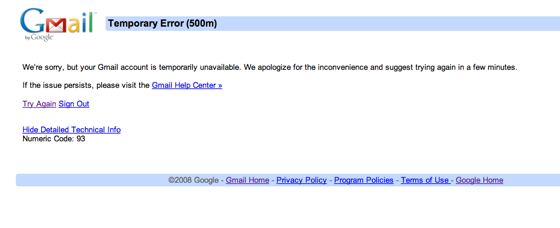
\includegraphics[width=120mm]{Imagens/gmailDown.png}
\caption{Add a single tag on all Gmail emails.\label{fig:gmailDown}}
\end{figure}

Dizer aqui que depois o MySQL lancou a versao com FTS. 
Dizer que o ES abre um mundo de oportunidades para analytics.

Dizer que uma das ameacas pode ser o fator de chegada das requests nos cenarios avaliados, que podem nao representar o real. 
% Dizer que dava pra ao inves de tempo os slas serem orientados a acuracia tambem. Dizer de um caso: imagine uma aplicacao que diz quantos pontos tem dentro de um poligono. Com o banco tal a acuracia eh de X. Com o banco Y a acuracia eh de Z.

% TODO: Fix References: https://www.evernote.com/l/AD9tKczyJiBK9KJkJ-s1eNh-AxhMlqz3SXA

% The boundaries of this work could then be broadened to support the conception of a SLA-Guided process to support the migration/replacement of sotware components based on the cloud in future works.
% Dizer tambem que o pessoal recomenda migrar pedacos de feature a feature, como nesse case do Coursera. https://tech.coursera.org/blog/2014/09/23/courseras-adoption-of-cassandra/
